\documentclass{article}
\usepackage[backend=biber, style=numeric, citestyle=numeric]{biblatex}
\addbibresource{ref.bib}
\usepackage{graphicx}
\usepackage{amsmath, bm, amssymb}
\usepackage{titlesec}
\usepackage{geometry}
\usepackage{fancyhdr}
\usepackage{xcolor}
\usepackage{algorithm}
\usepackage{algpseudocode}
\usepackage{hyperref}
\usepackage{caption}
\usepackage{subcaption}
\usepackage{color}
\definecolor{darkred}{rgb}{0.6,0.0,0.0}
\definecolor{darkgreen}{rgb}{0,0.50,0}
\definecolor{lightblue}{rgb}{0.0,0.42,0.91}
\definecolor{orange}{rgb}{0.99,0.48,0.13}
\definecolor{grass}{rgb}{0.18,0.80,0.18}
\definecolor{pink}{rgb}{0.97,0.15,0.45}

% listings
\usepackage{listings}

% General Setting of listings
\lstset{
  aboveskip=1em,
  breaklines=true,
  abovecaptionskip=-6pt,
  captionpos=b,
  escapeinside={\%*}{*)},
  frame=single,
  numbers=left,
  numbersep=15pt,
  numberstyle=\tiny,
}
% 0. Basic Color Theme
\lstdefinestyle{colored}{ %
  basicstyle=\ttfamily,
  backgroundcolor=\color{white},
  commentstyle=\color{green}\itshape,
  keywordstyle=\color{blue}\bfseries\itshape,
  stringstyle=\color{red},
}
% 1. General Python Keywords List
\lstdefinelanguage{PythonPlus}[]{Python}{
  morekeywords=[1]{,as,assert,nonlocal,with,yield,self,True,False,None,} % Python builtin
  morekeywords=[2]{,__init__,__add__,__mul__,__div__,__sub__,__call__,__getitem__,__setitem__,__eq__,__ne__,__nonzero__,__rmul__,__radd__,__repr__,__str__,__get__,__truediv__,__pow__,__name__,__future__,__all__,}, % magic methods
  morekeywords=[3]{,object,type,isinstance,copy,deepcopy,zip,enumerate,reversed,list,set,len,dict,tuple,range,xrange,append,execfile,real,imag,reduce,str,repr,}, % common functions
  morekeywords=[4]{,Exception,NameError,IndexError,SyntaxError,TypeError,ValueError,OverflowError,ZeroDivisionError,}, % errors
  morekeywords=[5]{,ode,fsolve,sqrt,exp,sin,cos,arctan,arctan2,arccos,pi, array,norm,solve,dot,arange,isscalar,max,sum,flatten,shape,reshape,find,any,all,abs,plot,linspace,legend,quad,polyval,polyfit,hstack,concatenate,vstack,column_stack,empty,zeros,ones,rand,vander,grid,pcolor,eig,eigs,eigvals,svd,qr,tan,det,logspace,roll,min,mean,cumsum,cumprod,diff,vectorize,lstsq,cla,eye,xlabel,ylabel,squeeze,}, % numpy / math
}
% 2. New Language based on Python
\lstdefinelanguage{PyBrIM}[]{PythonPlus}{
  emph={d,E,a,Fc28,Fy,Fu,D,des,supplier,Material,Rectangle,PyElmt},
}
% 3. Extended theme
\lstdefinestyle{colorEX}{
  basicstyle=\ttfamily,
  backgroundcolor=\color{white},
  commentstyle=\color{darkgreen}\slshape,
  keywordstyle=\color{blue}\bfseries\itshape,
  keywordstyle=[2]\color{blue}\bfseries,
  keywordstyle=[3]\color{grass},
  keywordstyle=[4]\color{red},
  keywordstyle=[5]\color{orange},
  stringstyle=\color{darkred},
  emphstyle=\color{pink}\underbar,
}





\geometry{left=1in, right=1in, top=1in, bottom=1in}

\definecolor{titlecolor}{RGB}{0, 0, 128}

\titleformat{\section}[block]{\normalfont\Large\bfseries\color{titlecolor}}{\thesection}{1em}{}
\titleformat{\subsection}[block]{\normalfont\large\bfseries\color{titlecolor}}{\thesubsection}{1em}{}

\pagestyle{fancy}
\fancyhf{}
\lhead{\scriptsize EEC 289A Assignment 1 Report}
\rhead{}
\cfoot{\thepage}

\begin{document}

\noindent
\textbf{\large EEC 289A Assignment 1 Report} \\
\textbf{\small Chenye Yang, Hanchu Zhou, Haodong Liang, Yibo Ma}



\section{Introduction}

In this project, we aim to do K-mean clustering on the patches from MNIST dataset, shown in Figure~\ref{fig:mnist}. After the clustering, we observe the results, and try to answer the following interesting questions:
\begin{enumerate}
    \item What is the change of the learned clusters when K increases from 100 - 10,000?
    \item How well one can reconstruct a 5x5 MNIST patch by the learned dictionary (clusters)?
    \item How many clusters does one need in order to cover the whole patch space?
    \item What are these clusters and do they have any interpretable meanings?
    \item How is one digit made from these clusters?
\end{enumerate}

\begin{figure}[htbp!]
    \centering
    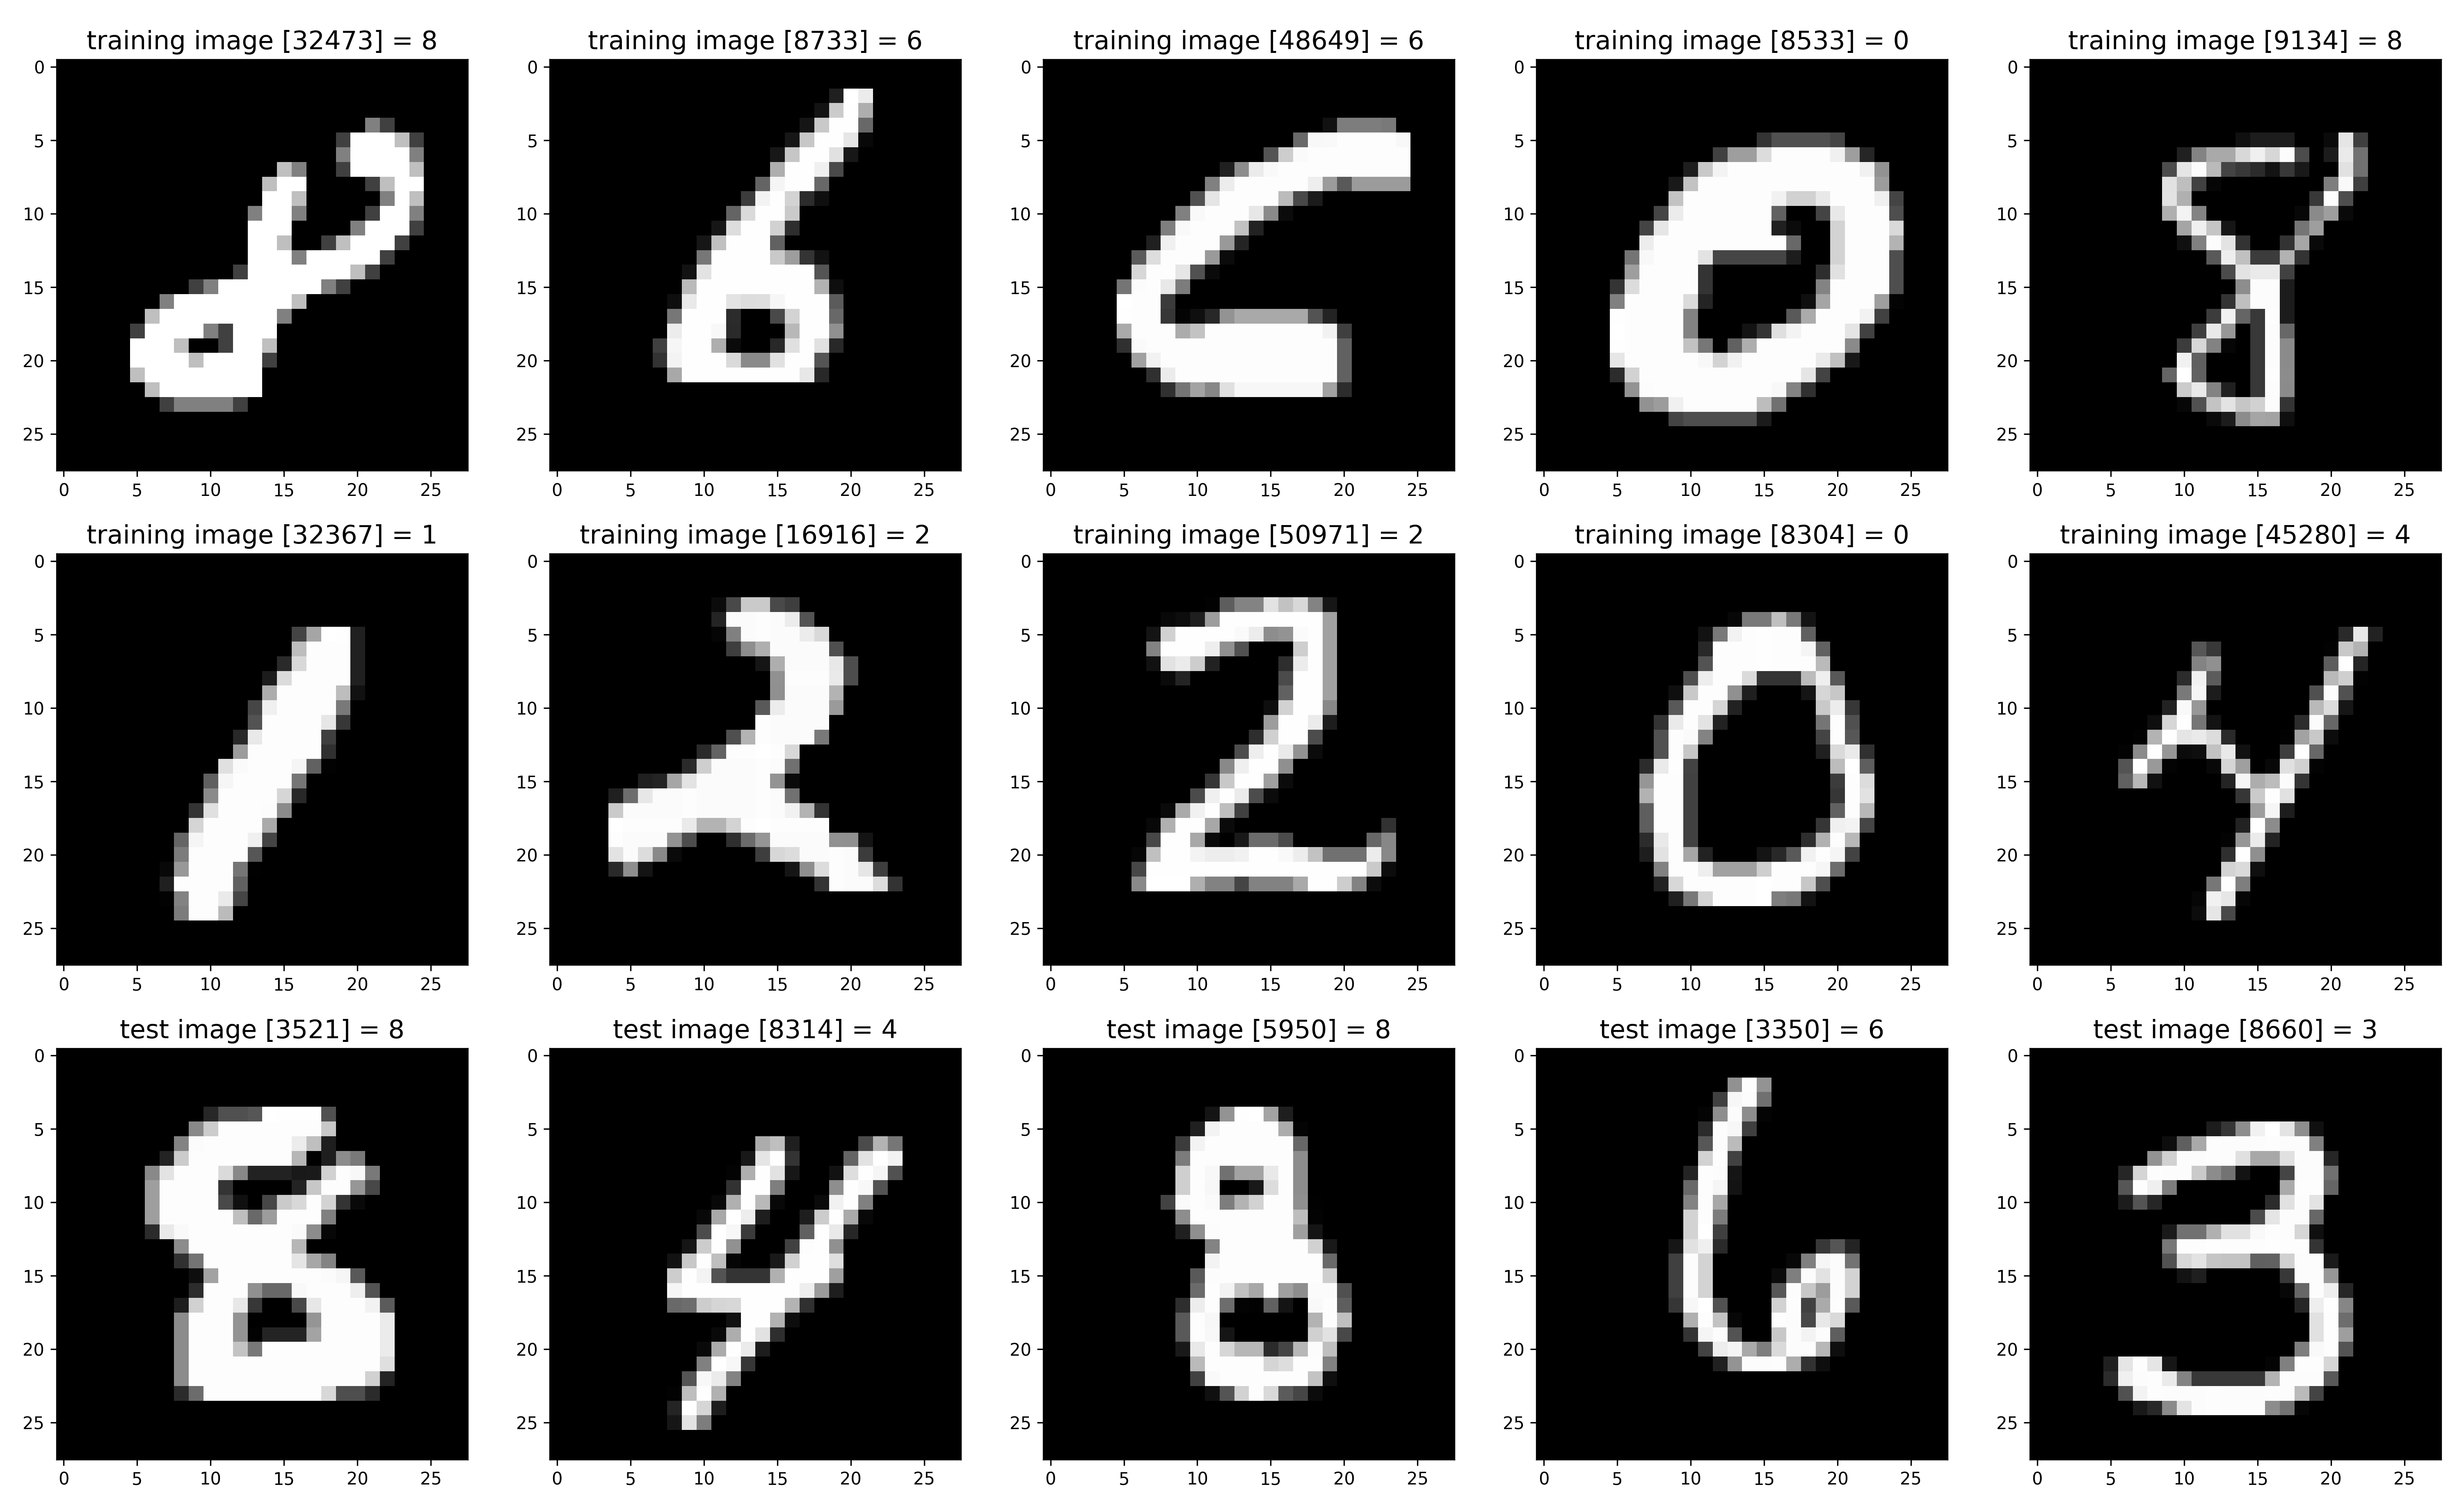
\includegraphics[width = 0.6 \textwidth]{../Result/mnist_images.png}
    \caption{Some examples of the MNIST dataset}
    \label{fig:mnist}
\end{figure}


\section{Methodology}
\subsection{Data Preprocessing}

We load the MNIST dataset ($28 \times 28$ handwritten digits)\footnote{Downloaded from \url{https://git-disl.github.io/GTDLBench/datasets/mnist_datasets/}}, including 60000 training images and 10000 testing images. 
The pixel values in each image are not normalized, and they range from 0 (black) to 255 (white).
Then, we extract the patches from the training images, by sliding a 5$\times$5 window over the images.
Therefore, for each handwritten digit, we will get $(28 -5 +1) \times (28 - 5 + 1)$ patches. 
Then we get rid of all the blank patches, leading to 20,074,704 non-blank patches in total.
Each patch is reshaped to a 25-dimensional vector, and we get a matrix $X \in R^{20,074,704 \times 25}$.


\subsection{K-mean clustering}

Once we get all the patches, we can do the K-mean clustering on the patches. 
The K-mean clustering is a method to partition the data into K clusters, where each data point belongs to the cluster with the nearest mean.
Although there is a wildly used K-means algorithm in library \textit{scikit learn}\footnote{\url{https://scikit-learn.org/stable/modules/generated/sklearn.cluster.KMeans.html}}, 
we also implement the K-means clustering algorithm using PyTorch, hoping to achieve acceleration by using Nvidia CUDA\footnote{\url{https://pytorch.org/docs/stable/cuda.html}} or Apple MPS\footnote{\url{https://developer.apple.com/metal/pytorch/}}, 
which is shown in the Algorithm~\ref{alg:kmeans}.

We define that:

\begin{itemize}
    \item $K$: Number of the clustering 
    \item $C$: Centroids of the clustering
    \item $P$: The 5 $\times$ 5 patch
    \item $X$: The entire dataset of patches with size $20,074,704 \times 25$
\end{itemize}

\begin{algorithm}
\caption{PyTorch K-means Clustering for $5 \times 5$ Patches}\label{alg:kmeans}
\begin{algorithmic}[1]
\Procedure{KMeansPatches}{$Patches, K$}
    \State $X \gets \text{Reshape each patch } P \text{ in } Patches \text{ to } R^{25}$ \Comment{No normalization}
    \State Initialize $C$ random $K$ data points from $X$
    \State $C_{\text{old}} \gets \text{Copy of } C$
    \Repeat
        \State Compute distances from each vector $X_i$ in $X$ to each centroid in $C$
        \State Assign each vector $X_i$ to the closest centroid
        \For{$j \gets 1$ \text{to} $K$}
            \If{$\text{Count}(X_i \text{ assigned to } C_j) = 0$}
                \State Randomly reinitialize centroid $C_j$ from $X$
            \Else
                \State Update centroid $C_j$ by calculating the mean of all vectors assigned to $C_j$
            \EndIf
        \EndFor
        \State $C_{\text{new}} \gets \text{Copy of } C$
        \State $C_{\text{move}} \gets \text{norm}(C_{\text{new}} - C_{\text{old}})$
        \State $C_{\text{old}} \gets C_{\text{new}}$
    \Until{$C_{\text{move}} < \text{tolerance}$}
    \State \Return Updated centroids and cluster labels
\EndProcedure
\end{algorithmic}
\end{algorithm}


\subsection{Reconstruction}

After the clustering, we can use the centroids to reconstruct the original digits, as shown in Algorithm~\ref{alg:reconstruct}.
The reconstruction is done by assigning each non-blank patch to the nearest centroid, and keep the blank patches as zeros.
Because of the overlap of the patches, we will have multiple centroids assigned to the same pixel.
Thus, we need a count matrix to record the number of how many centroids are assigned to each pixel.
Finally, we average the value of each pixel to get the reconstructed digit.

Some notations in this algorithm:

\begin{itemize}
    \item $POS$: The position indices of a specific patch
    \item $D$: The ground truth of the handwritten digit 
    \item $\hat{D}$: The reconstructed result of $D$ according to the K-mean clustering centroids
\end{itemize}


\begin{algorithm}
\caption{Reconstruct Handwritten Digit Images}\label{alg:reconstruct}
\begin{algorithmic}[1]
\Procedure{ReconstructDigit}{$D, K, Model$}
    \State $P \gets \text{empty list to store patches}$
    \State $Pos \gets \text{empty list to store position indices}$
    \For{$i \gets 1 \text{ to } 24$} \Comment{28 - 5 + 1 = 24}
        \For{$j \gets 1 \text{ to } 24$}
            \State $patch \gets D[i:i+5, j:j+5]$
            \If{$\text{not all zeros in } patch$}
                \State $P.\text{append}(patch.flatten())$
                \State $Pos.\text{append}((i, j))$
            \EndIf
        \EndFor
    \EndFor
    \State $X \gets \text{stack of patches in } P$
    \State $Labels \gets Model.\text{predict}(X)$ \Comment{Assign patches to centroids}
    \State $\hat{D} \gets \text{zero matrix of the same size as } D$ \Comment{Initialize reconstructed digit with zeros}
    \State $Count \gets \text{zero matrix of the same size as } D$ \Comment{Initialize Count matrix with zeros}

    \For{$k \gets 0 \text{ to } \text{len}(P)-1$}
        \State $pos \gets Pos[k]$
        \State $cluster \gets Labels[k]$
        \State $centroid \gets Model.cluster\_centers_[cluster].reshape(5, 5)$
        \State $\hat{D}[pos[0]:pos[0]+5, pos[1]:pos[1]+5] \gets \hat{D}[pos[0]:pos[0]+5, pos[1]:pos[1]+5] + centroid$
        \State $Count[pos[0]:pos[0]+5, pos[1]:pos[1]+5] \gets Count[pos[0]:pos[0]+5, pos[1]:pos[1]+5]+1$
    \EndFor
    \State $Count[Count == 0] = 1$  \Comment{Avoid division by 0}

    \State \Return $\hat{D}/Count$
\EndProcedure
\end{algorithmic}
\end{algorithm}



\section{Experiment Results}\label{sec:experiment}

\subsection{Clustering Results with Different $K$}
We conducted the K-mean clustering on the patches with different $K$ values, where:
\[K = 100, 200, 300, \dots, 900, 1000, 2000, \dots, 9000, 10000. \]
Some results of the patches and the corresponding centroids are shown in the following Figures~\ref{fig:patches-100}-\ref{fig:patches-10000}.


\begin{figure}[htbp!]
    \centering
    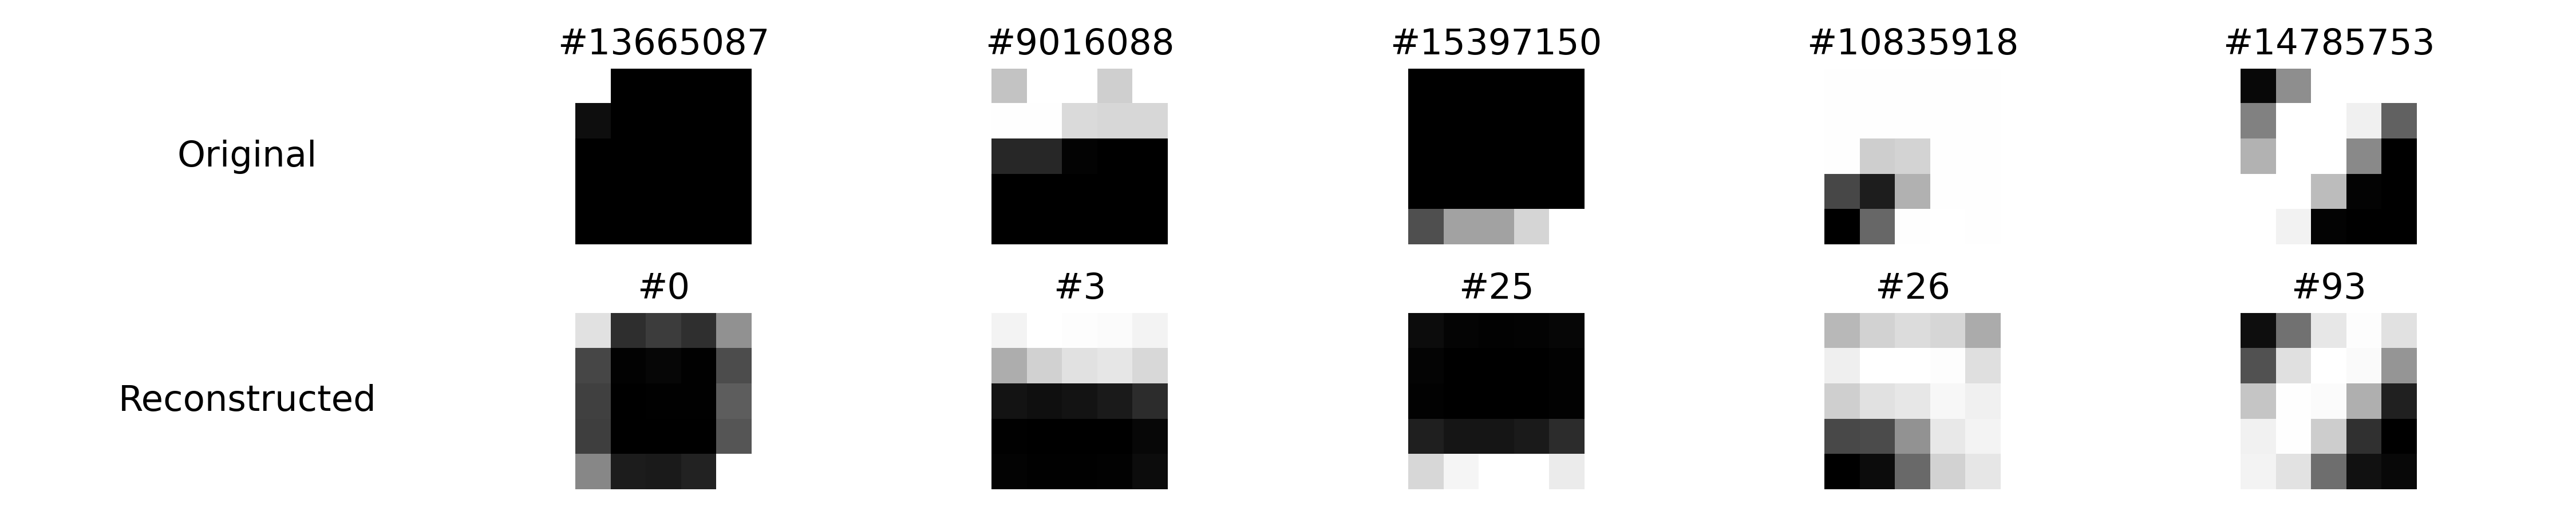
\includegraphics[width = 0.9 \textwidth]{../Result/Patches/100-clusters-reconstruction.png}
    \caption{The patch and corresponding centroid when $K = 100$}
    \label{fig:patches-100}
\end{figure}


\begin{figure}[htbp!]
    \centering
    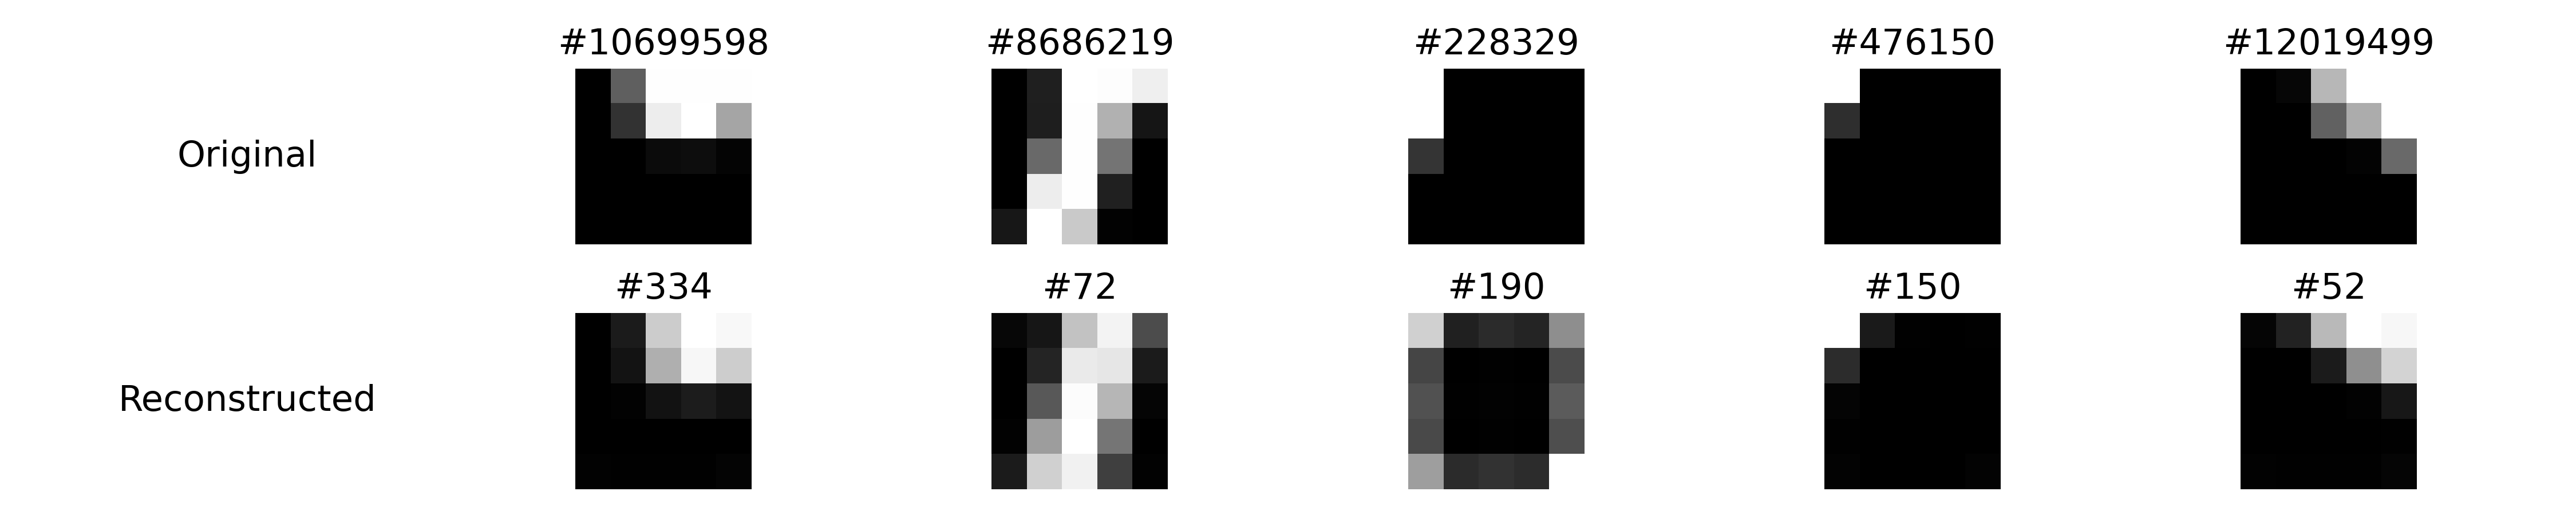
\includegraphics[width = 0.9 \textwidth]{../Result/Patches/400-clusters-reconstruction.png}
    \caption{The patch and corresponding centroid when $K = 400$}
    \label{fig:patches-400}
\end{figure}
% \clearpage


\begin{figure}[htbp!]
    \centering
    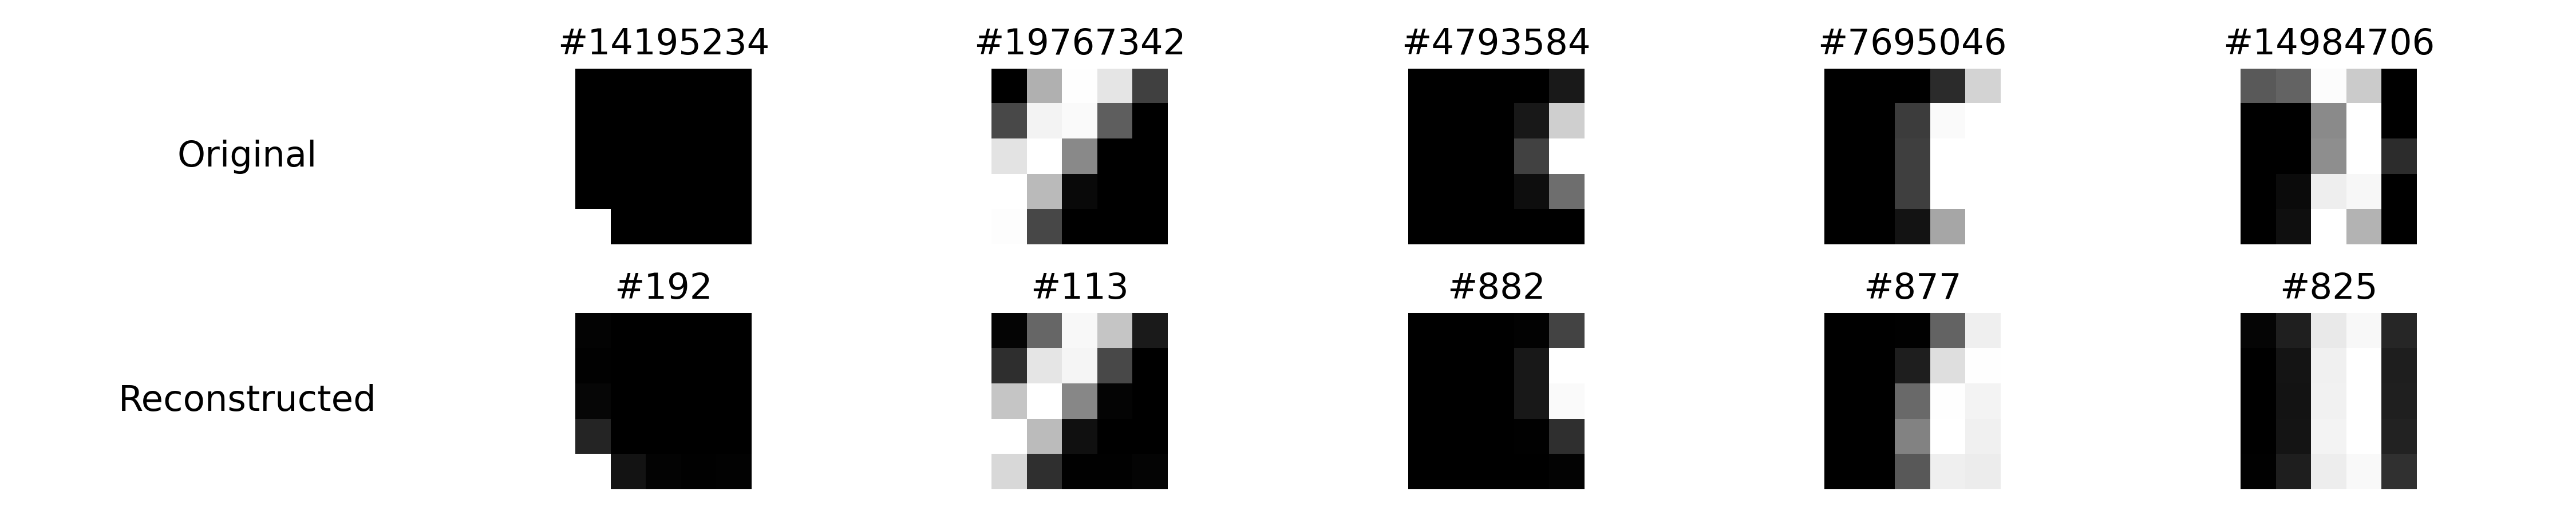
\includegraphics[width = 0.9 \textwidth]{../Result/Patches/1000-clusters-reconstruction.png}
    \caption{The patch and corresponding centroid when $K = 1000$}
    \label{fig:patches-1000}
\end{figure}
% \clearpage


\begin{figure}[htbp!]
    \centering
    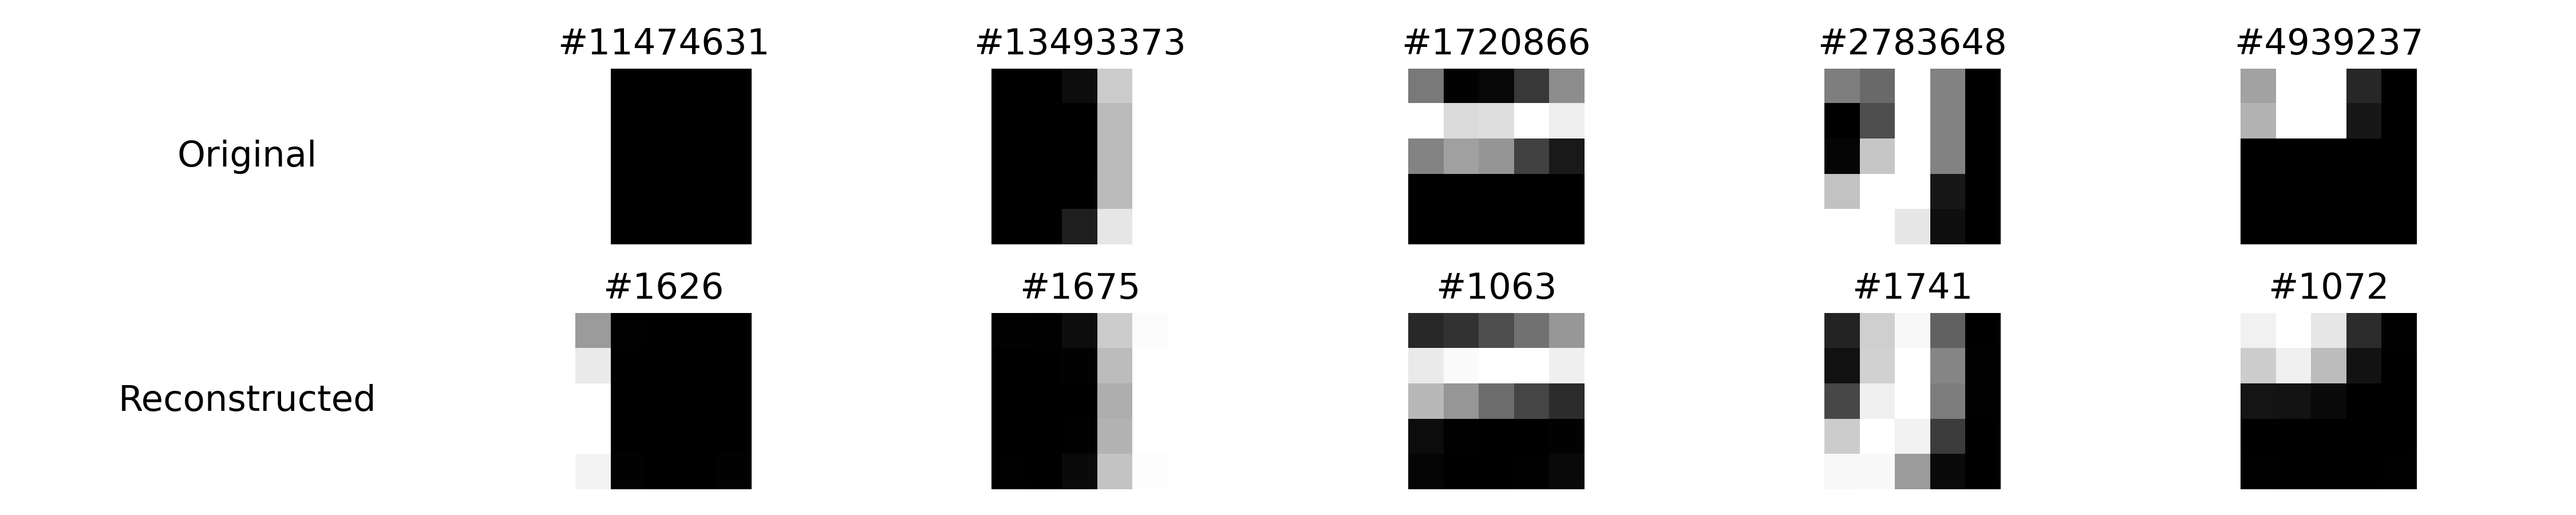
\includegraphics[width = 0.9 \textwidth]{../Result/Patches/2000-clusters-reconstruction.png}
    \caption{The patch and corresponding centroid when $K = 2000$}
    \label{fig:patches-2000}
\end{figure}

\begin{figure}[htbp!]
    \centering
    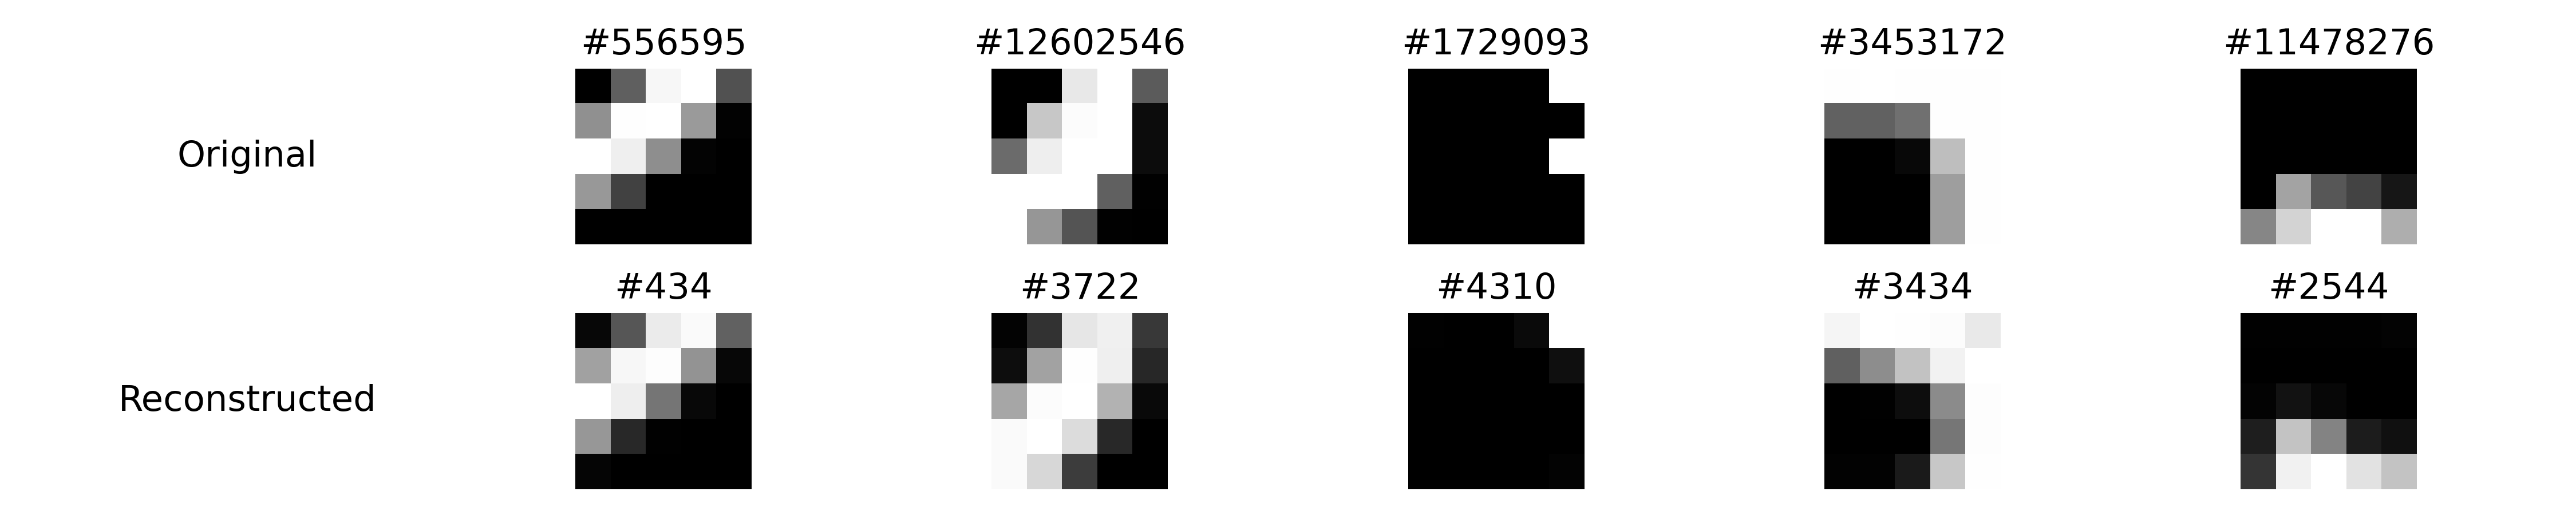
\includegraphics[width = 0.9 \textwidth]{../Result/Patches/5000-clusters-reconstruction.png}
    \caption{The patch and corresponding centroid when $K = 5000$}
    \label{fig:patches-5000}
\end{figure}


\begin{figure}[htbp!]
    \centering
    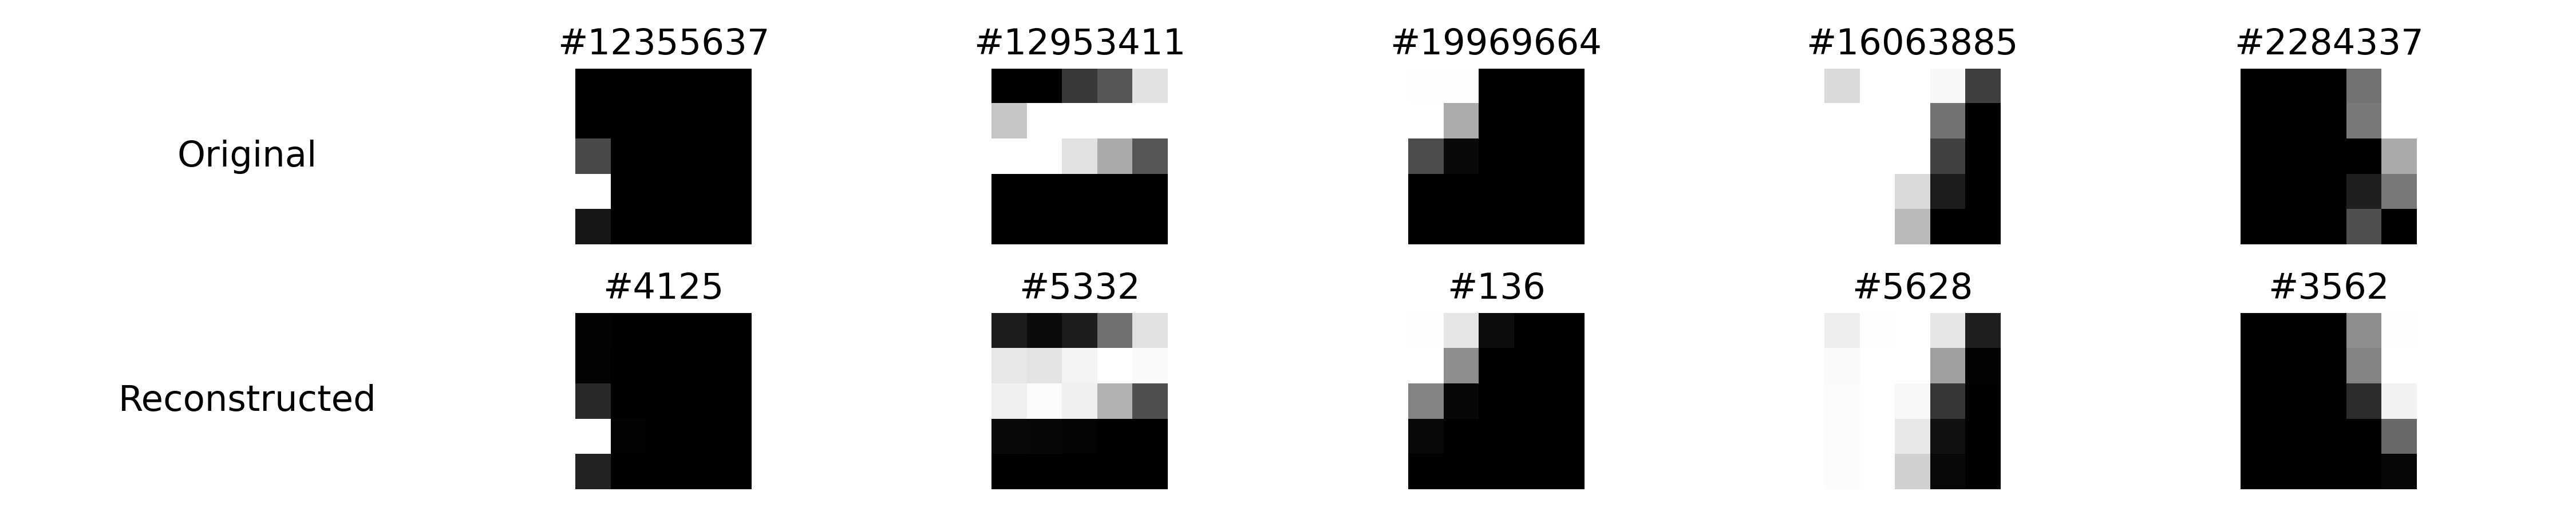
\includegraphics[width = 0.9 \textwidth]{../Result/Patches/10000-clusters-reconstruction.png}
    \caption{The patch and corresponding centroid when $K = 10000$}
    \label{fig:patches-10000}
\end{figure}

Moreover, we plot the Mean Squared Error (MSE) between the original patches and the reconstructed patches (centroids) with different $K$ values, as shown in Figure~\ref{fig:mse-k}.

\begin{figure}[htbp!]
    \centering
    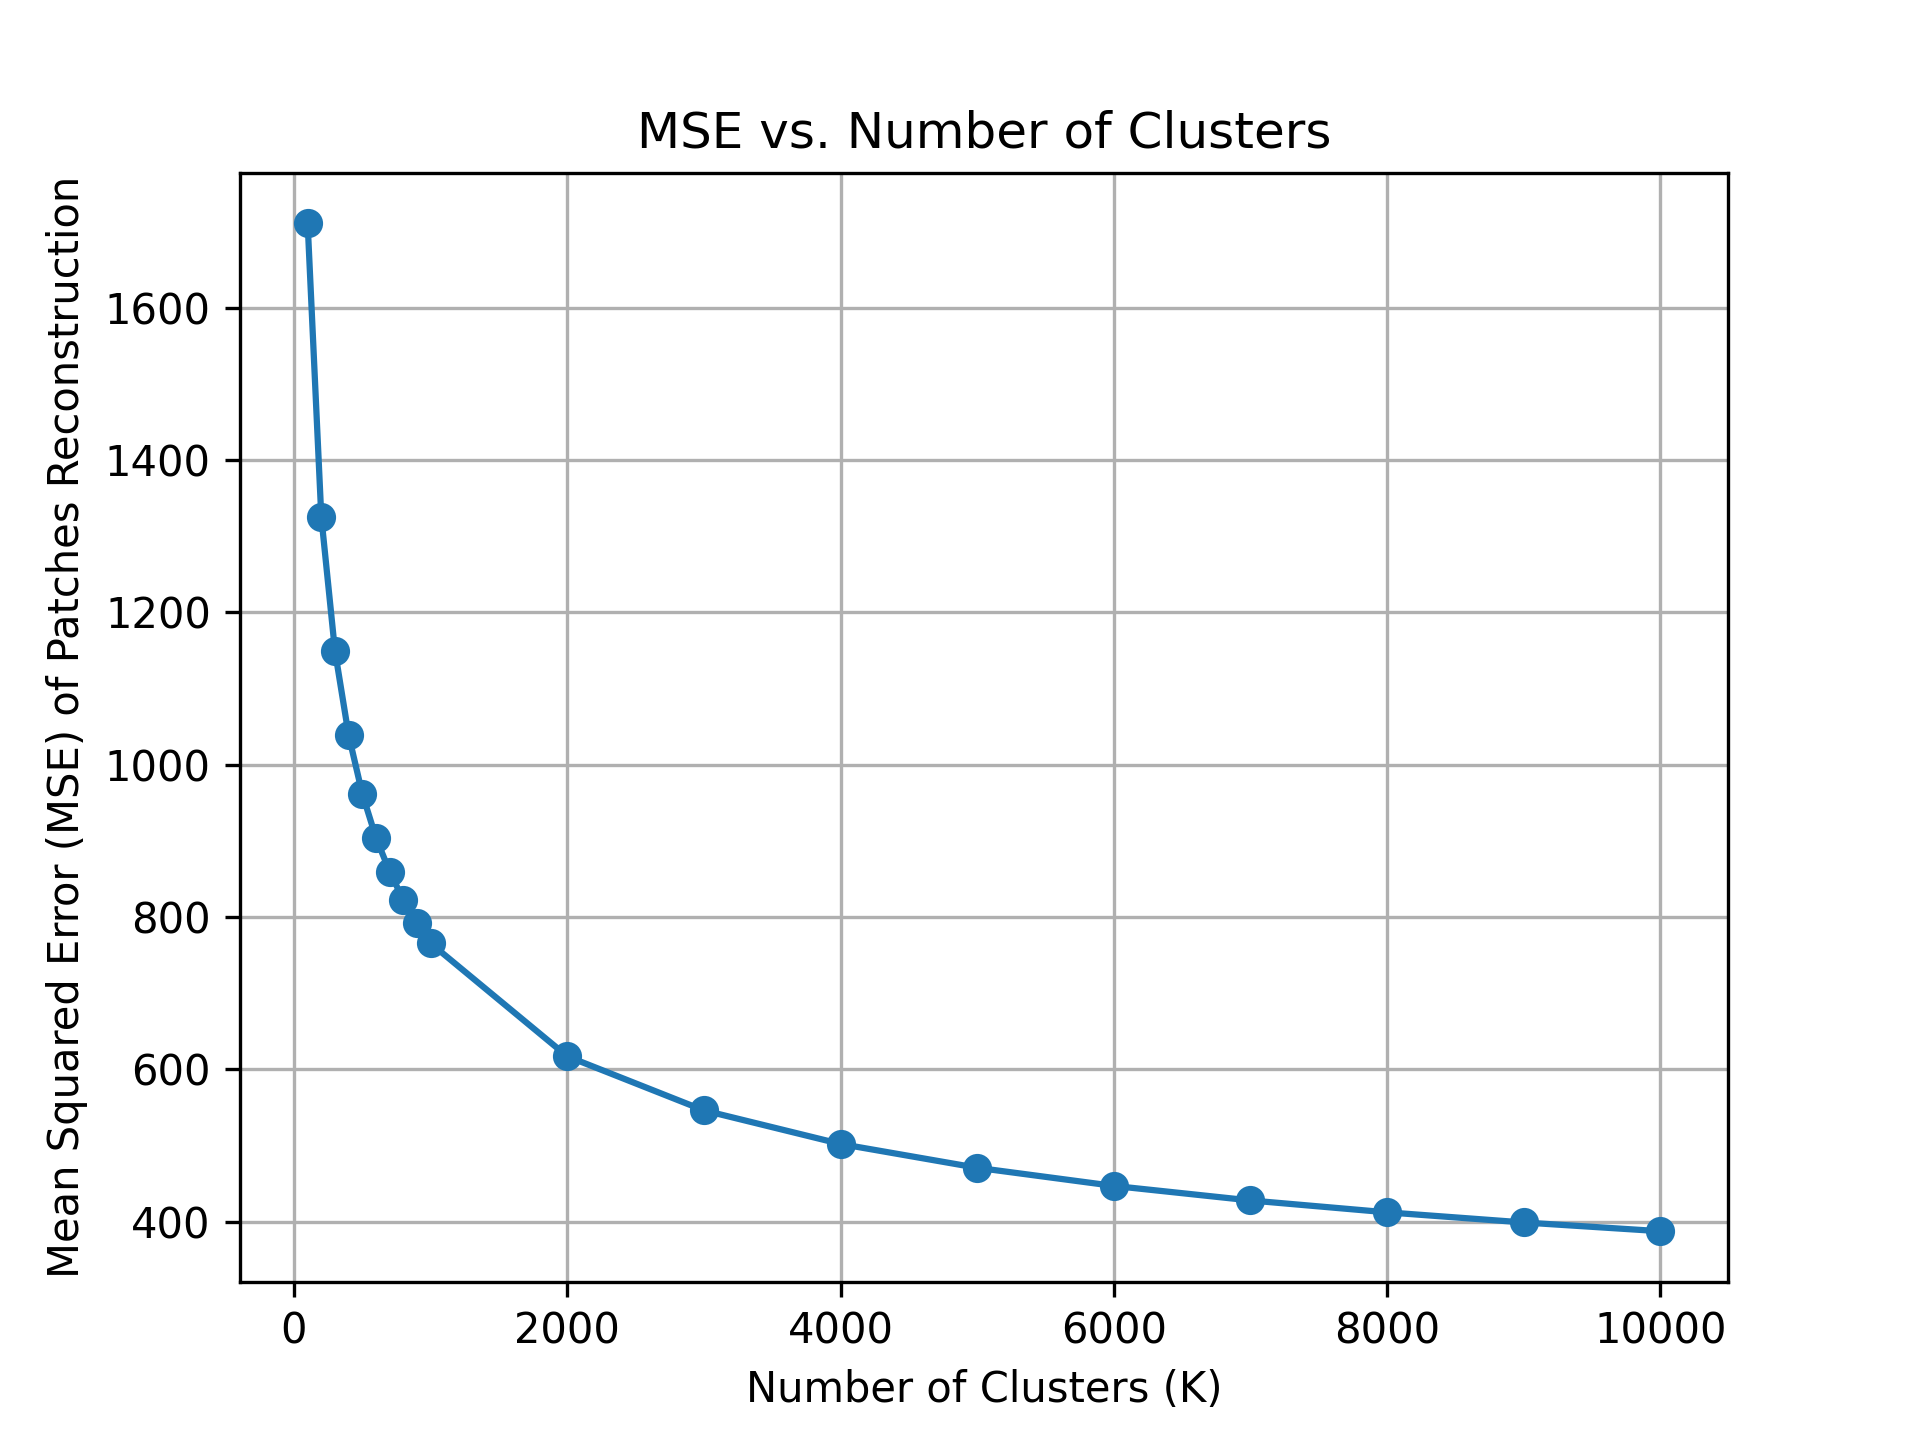
\includegraphics[width = 0.6 \textwidth]{../Result/Patches/MSE_vs_K.png}
    \caption{MSE with different clustering number}
    \label{fig:mse-k}
\end{figure}

With the results above, we can observe that:
\begin{itemize}
    \item \textcolor{red}{Question 1:} As K increases, the learned clusters become more and more detailed and similar to the original patches.
    \item \textcolor{red}{Question 2:} With the increase of K, one can reconstruct the patches more accurately. For example, when $K = 100$, the reconstructed patches are not very similar, but when $K = 10000$, the reconstructed patches are very similar to the original patches.
    \item \textcolor{red}{Question 3:} The MSE decreases as K increases, however, the decreasing rate becomes slower when K is large. By elbow method, we can find that the optimal K is around 2000. So we need 2000 clusters to cover the whole patch space, considering the trade-off between the clustering performance and the computational cost.
\end{itemize}


\subsection{What are the centroids}

In addition to the clustering performance, we also want to understand the meaning of the clusters or centroids. 
Here we show all the centroids when using $K = 100$ and $K = 1000$ in Figure~\ref{fig:centroids-100-1000}.


\begin{figure}[htbp!]
    \centering
    % Only two subfigures for K=100 and K=10000
    \begin{subfigure}[b]{0.48\textwidth}
        \centering
        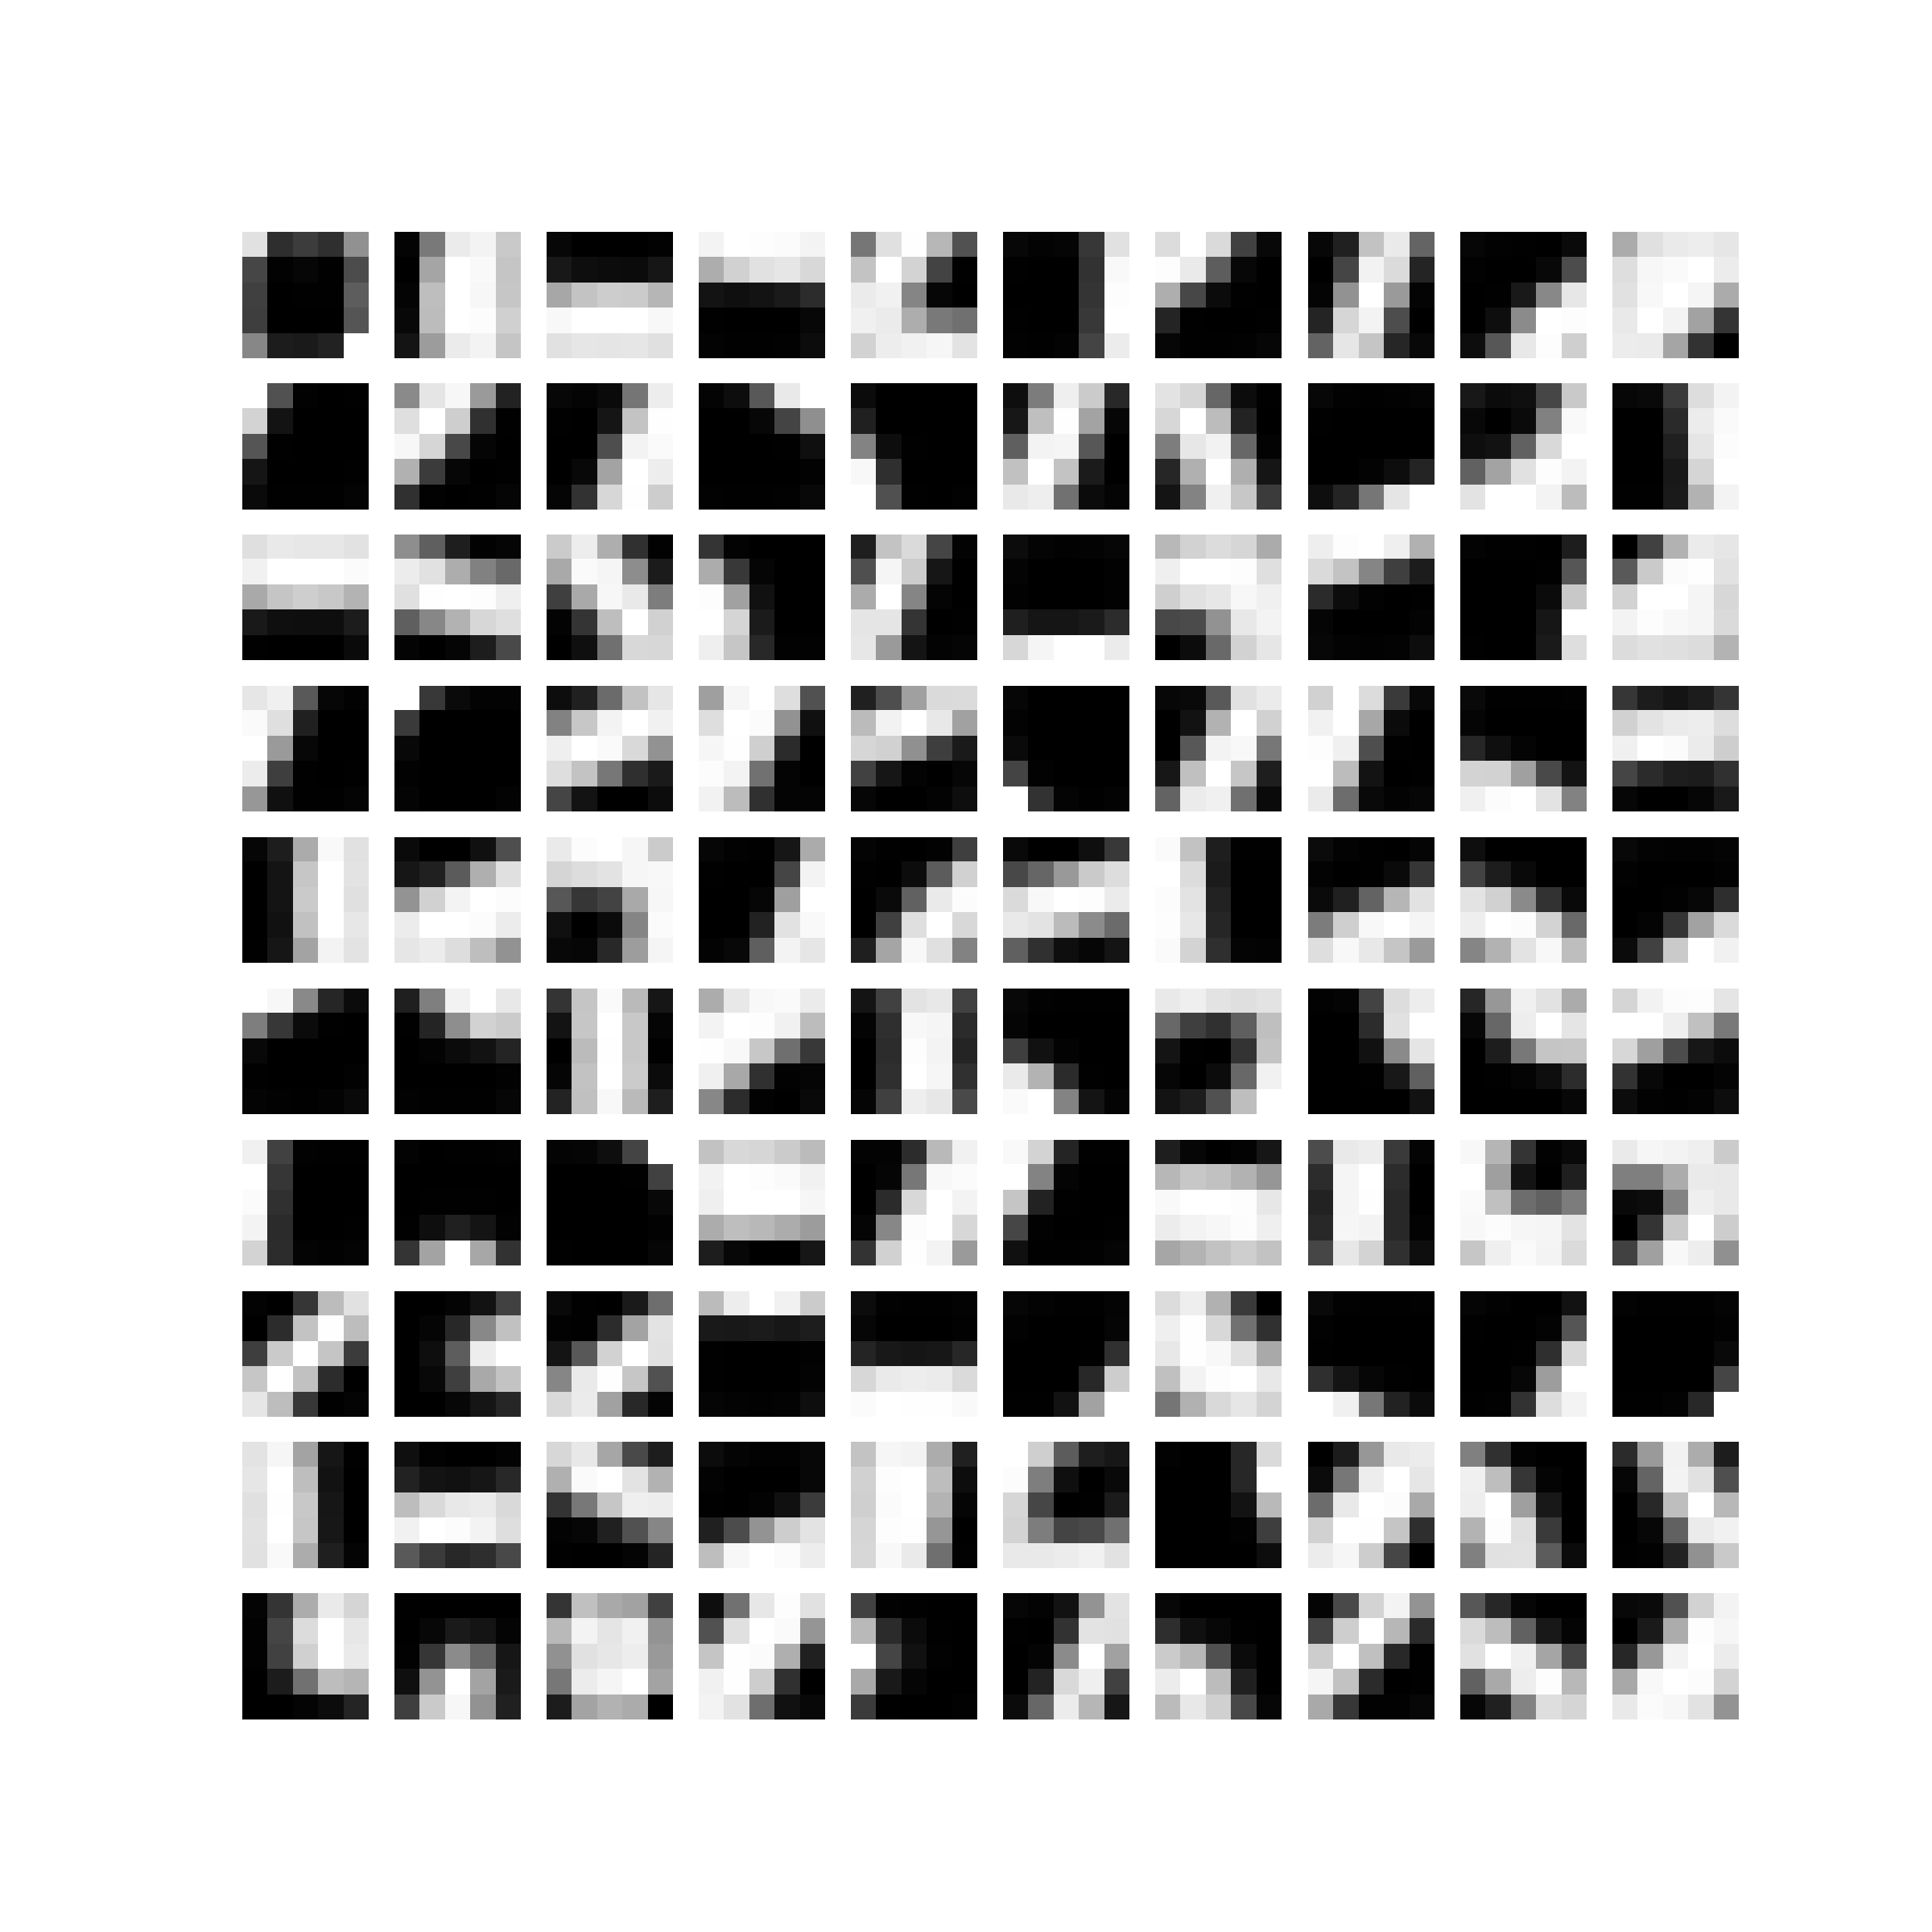
\includegraphics[width=\textwidth]{../Result/Centroids/100-clusters-centroids.png}
        \caption{$K = 100$}
        \label{fig:100-centroids}
    \end{subfigure}
    \hfill
    \begin{subfigure}[b]{0.48\textwidth}
        \centering
        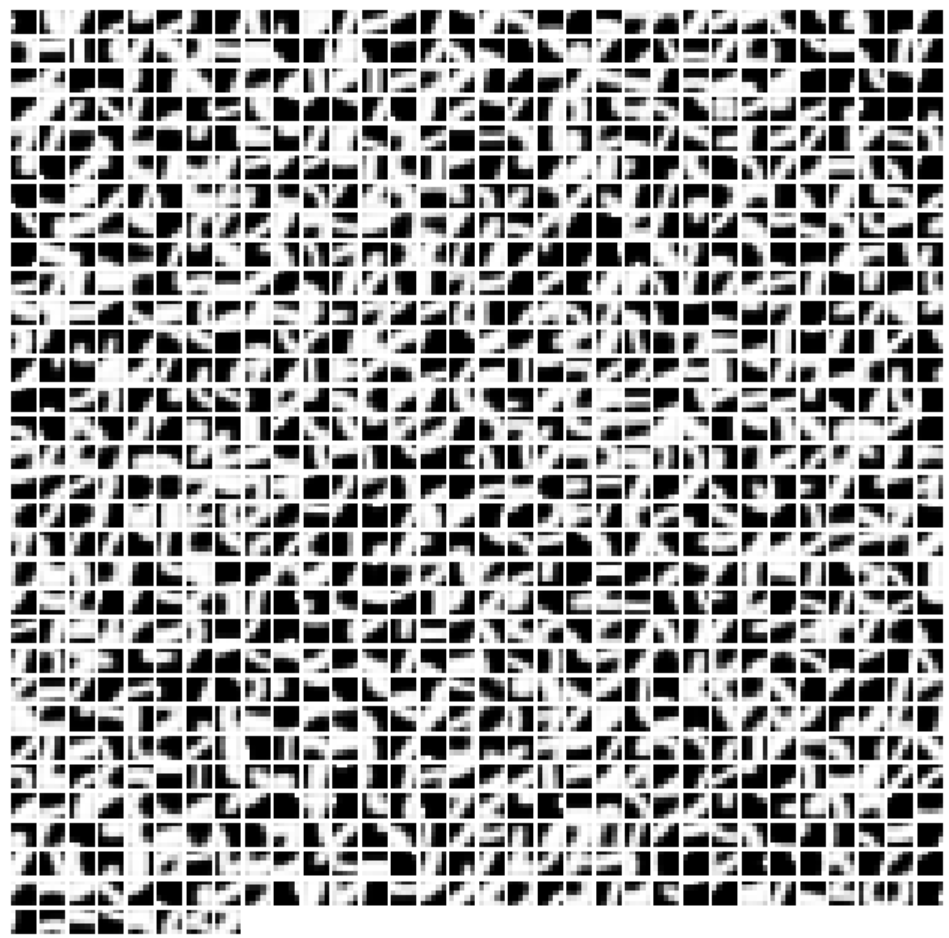
\includegraphics[width=\textwidth]{../Result/Centroids/Screenshot 2024-04-19 231953.png}
        \caption{$K = 1000$}
        \label{fig:1000-centroids}
    \end{subfigure}
    \caption{Visual representation of cluster centroids for $K = 100$ and $K = 1000$}
    \label{fig:centroids-100-1000}
\end{figure}

\textcolor{red}{Question 4:} From the results, we can see that the centroids of these clusters are actually the patterns of the handwritten digits. Specifically, they are the edges, corners, and other features of the digits.


\subsection{Reconstruct a Digit}
In this part, we show the reconstruction results of the handwritten digits from both the training set and testing set, by using the learned centroids, as in Figures~\ref{fig:digit-train} and~\ref{fig:digit-test}.

\begin{figure}[htbp!]
    \centering
    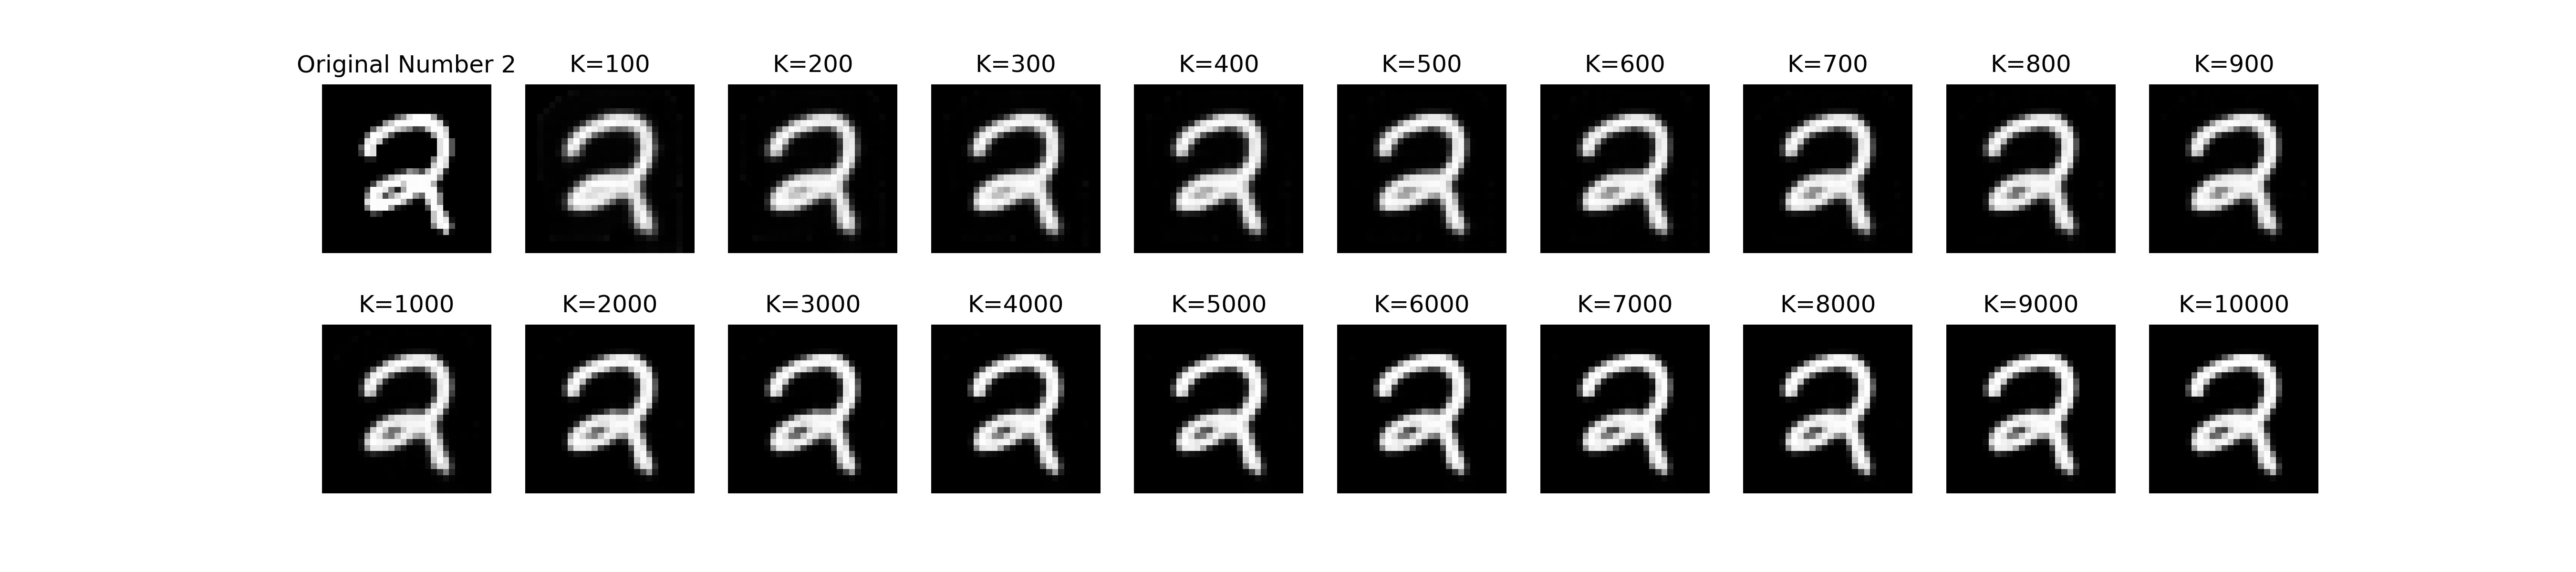
\includegraphics[width = \textwidth]{../Result/Digits/reconstruct-train-digit.png}
    \caption{Reconstruction of digit 2 with different $K$}
    \label{fig:digit-train}
\end{figure}
\begin{figure}[htbp!]
    \centering
    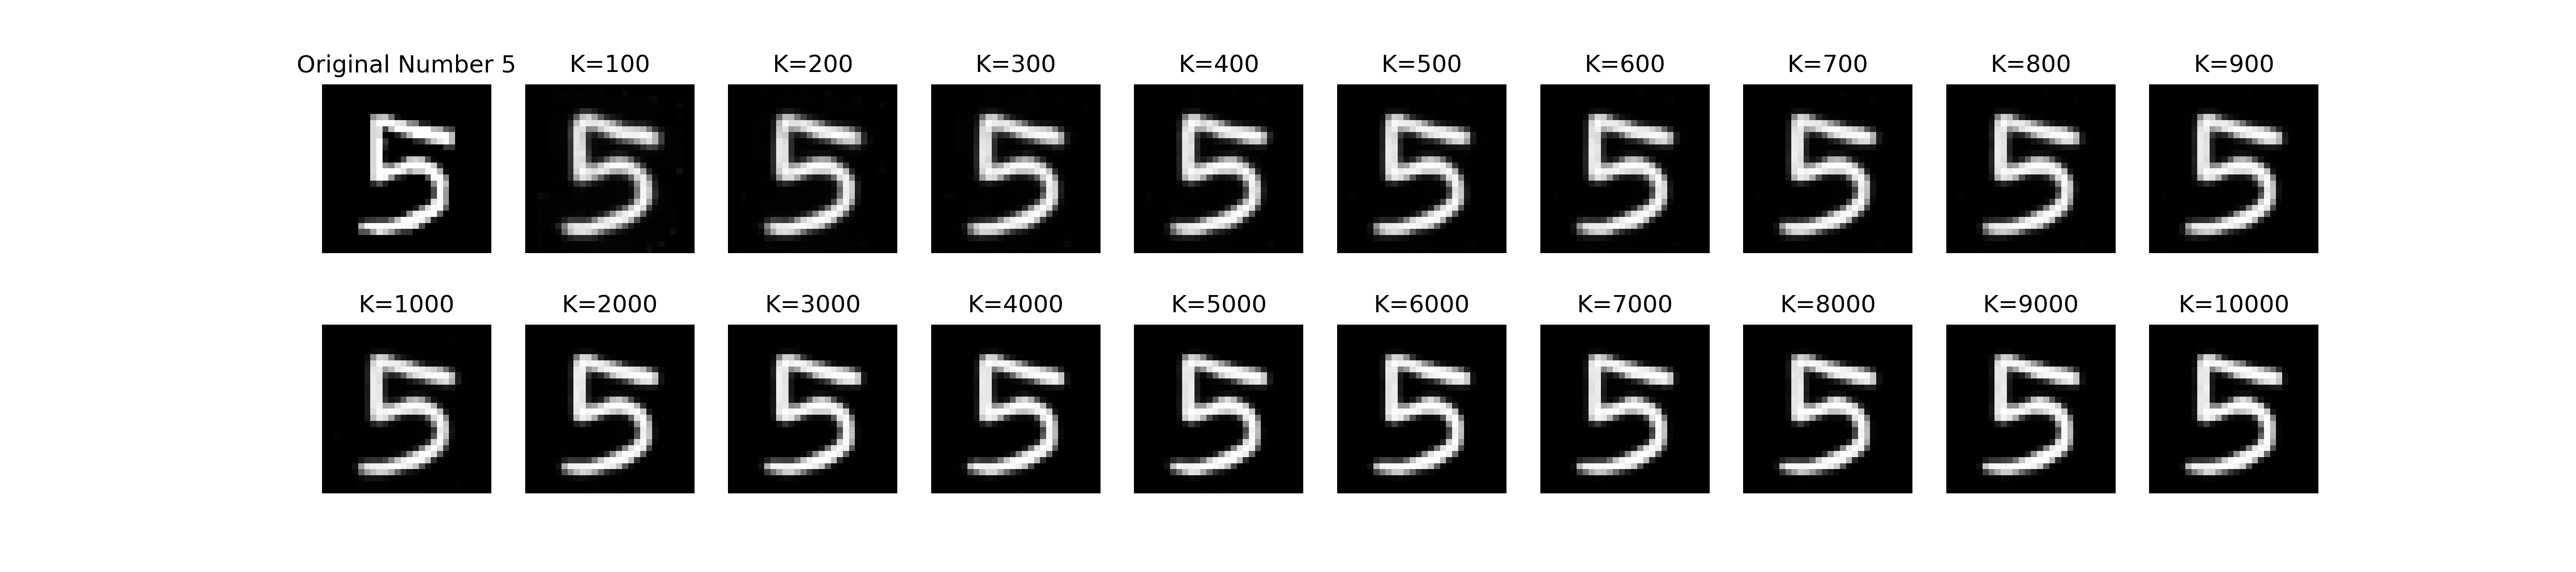
\includegraphics[width = \textwidth]{../Result/Digits/reconstruct-test-digit.png}
    \caption{Reconstruction of digit 5 with different $K$}
    \label{fig:digit-test}
\end{figure}

From the results, we can observe that the reconstructed digits are very vague when $K = 100$, but they become more and more clear as $K$ increases. 
When $K = 10000$, the reconstructed digits are very similar to the original digits. 
\textcolor{red}{Question 5:} This indicates that the digits are constructed from the detailed features of itself, such as the edges, corners, and other features.
One digit is just a linear combination of these features / centroids/ clusters, and the more clusters we have, the more accurate the reconstruction will be.

\section{Conclusion}

In this project, we use K-mean clustering to learn the dictionary (cluster) of the $5\times 5$ patches of the MNIST dataset, and analyze the performance with different K. We can now answer the questions we raised at the beginning:

\begin{itemize}
    \item When K increases, the learned clusters contain more detailed information on each figure element.
    \item As shown in Figure~\ref{fig:patches-100}-\ref{fig:patches-10000}, a $5\times 5$ MNIST patch can be well reconstructed by the learned clusters. The reconstruction quality is better when K is large.    
    \item Ideally, we want the number of clusters to be as large as possible. However, Figure~\ref{fig:mse-k} implies that the marginal return is lower when $K>2000$, and in practice the training time is huge when K is large. So $K=2000$ would be a reasonable choice.
    \item The visualization of these clusters are shown in Figure~\ref{fig:centroids-100-1000}. These clusters are the "elements" of each handwritten digits. They cover some common patterns such as lines, curves, and dots.
    \item The reconstructed digits are shown in Figure~\ref{fig:digit-train}-\ref{fig:digit-test}. With K=100, the reconstructed digits are already recognizable. The reconstruction quality is better with a larger K.
\end{itemize}

\newpage
\section*{Appendix}
\lstinputlisting[language=PythonPlus]{../Code/mnist_data_loader.py}
\lstinputlisting[language=PythonPlus]{../Code/extract_patches.py}
\lstinputlisting[language=PythonPlus]{../Code/kmeans_pytorch.py}
\lstinputlisting[language=PythonPlus]{../Code/run_kmeans.py}
\lstinputlisting[language=PythonPlus]{../Code/evaluate_kmeans.py}
\lstinputlisting[language=PythonPlus]{../Code/reconstruct_digits.py}


% \printbibliography
\end{document}
